%%%%%%%%%%%%%%%%%%%%%%%%%%%%%%%%%%%%%%%%%%%%%%%%%%%%%%%%%%%%%%%%%%%%%%%%%
%%   CHAPTER: THE 0E0P METACELL
%%%%%%%%%%%%%%%%%%%%%%%%%%%%%%%%%%%%%%%%%%%%%%%%%%%%%%%%%%%%%%%%%%%%%%%%%

\renewcommand{\chapterfolder}{0e0p/}
\chapterimage{cover/0e0p}
\chapter{The 0E0P Metacell}\label{chp:0e0p}\index{0E0P metacell}


\vspace*{-0.4in}
\epigraph{If you couldn't predict what [Life] did then probably that's because it's capable of doing anything.}{John H. Conway}
\vspace*{0.15in}


\noindent In the previous chapter, we introduced universal construction and presented several adjustable spaceships based on it. In this chapter, we explore a more complex application of universal construction: a self-reproducing pattern that interacts with nearby copies of itself so as to emulate Conway's Game of Life, or a different cellular automaton, on a much larger and slower scale.

Specifically, we construct a pattern called the \textbf{0E0P metacell},\footnote{Constructed by Adam P.~Goucher from 2014 to November 2018. The acronym ``0E0P'' stands for ``(State) 0 Encoded by 0 Population'', in reference to the fact that its ``off'' state is just a metacell-sized region of empty space---its most remarkable property, which is not shared by any metacell that came before it (see Section~\ref{sec:0e0p_history}).} which has the property that if we arrange copies of it on the Life plane then, at a zoomed-out macroscopic scale, it evolves in the same way that the corresponding arrangement of cells would evolve. For example, if we place five copies of this metacell in the Life plane in the formation of a glider, as illustrated in Figure~\ref{fig:0e0p_glider}, then we indeed get a spaceship that travels like a glider (but much more slowly).

\begin{figure}[!htb]
	\centering
	\embedlink{0e0p_glider}{\vcenteredhbox{\patternimg{0.129}{0e0p_glider_0}} \vcenteredhbox{\color{black}{$\xrightarrow{\text{\clock{4}{45} $2^{36}$}}$}} \vcenteredhbox{\patternimg{0.129}{0e0p_glider_236}}}
	\caption{A \textbf{metaglider}\index{metaglider} made up of five copies of the 0E0P metacell, each of which is $2^{18} \times 2^{18}$ and logically makes up one ``cell''. It travels in much the same way as a glider, but $2^{36}$ times as slowly.}\label{fig:0e0p_glider}
\end{figure}

A meta-fied pattern like this is roughly $2^{18} = 262{\thousep}144$ times as large as the original pattern that it is based on, and it runs $2^{36} = 68{\thousep}719{\thousep}476{\thousep}736$ times as slowly. Indeed, the 0E0P metacell is so much larger and slower than any other pattern that we have seen in this book that evolving the metaglider from Figure~\ref{fig:0e0p_glider} through four ``metagenerations'' (i.e., $4 \times 2^{36}$ generations), to see that it really is a spaceship, would take a couple of years on a modern desktop computer via standard Life simulation algorithms.\footnote{The fastest ``standard'' Life simulation algorithm is \textbf{HashLife} \cite{Gos84}, which is fast enough to run any of the patterns that we saw earlier in this book---even huge ones like the $\pi$ calculator and the Gemini spaceship. To run patterns that use huge streams of gliders (like the 0E0P metacell) more efficiently, Adam P.~Goucher developed a new \textbf{StreamLife} algorithm, but even it would require several months to evolve a metaglider through four metagenerations.}\index{HashLife}\index{StreamLife}

While emulating Life within Life perhaps does not seem as remarkable a feat as some of the other things we have achieved over the past three chapters, what really makes the 0E0P metacell shine is that it can actually emulate a huge variety of 2D cellular automata besides Life as well. As a result, any pattern from one of those other cellular automata can be straightforwardly ``imported'' into Life simply by meta-fying it, thus giving us exotic new types of patterns that were previously not known how to construct.

To illustrate this phenomenon, consider the cellular automaton that has all the same rules as Life, plus the additional rule that a dead cell comes to life if it has exactly $6$ live neighbors (i.e., the Life-like cellular automaton with rulestring\index{rulestring} \texttt{B36/S23}). This cellular automaton is called \textbf{HighLife},\index{HighLife} and it is interesting for the fact that it has a simple \textbf{replicator}:\index{replicator (pattern)} a pattern that produces arbitrarily many copies of itself, as illustrated in Figure~\ref{fig:highlife_replicator}.

\begin{figure}[!htb]
	\centering
	\embedlink{highlife_replicator}{\vcenteredhbox{\patternimg{0.122}{highlife_replicator_0}} \vcenteredhbox{\genarrow{12}} \vcenteredhbox{\patternimg{0.122}{highlife_replicator_12}} \vcenteredhbox{\genarrow{12}} \vcenteredhbox{\patternimg{0.122}{highlife_replicator_24}} \vcenteredhbox{\genarrow{12}} \vcenteredhbox{\patternimg{0.122}{highlife_replicator_36}}}
	\caption{A \textbf{replicator} in the HighLife (\texttt{B36/S23}) Life-like cellular automaton that duplicates itself every $12$~generations. Found by Nathan Thompson in February 1994.}\label{fig:highlife_replicator}
\end{figure}

After this replicator copies itself the first time, each of its copies attempt to do the same. However, since these copies are right next to each other, two of \emph{their} copies attempt to occupy the same space, and instead annihilate each other (while their other copies are successfully created farther away). This behavior repeats forever: every $12$~generations, if there is space for a copy of this replicator then it is made, but two copies being made at the same spot at the same time mutually annihilate. The result is that after $n$ replication cycles (i.e., at generation $12n$), the number of replicators is exactly $2^{B(n)}$, where $B(n)$ is the \textbf{binary weight}\index{binary weight} of $n$: the number of ``1'' bits in its binary representation.

Since we're using HighLife's rules that require birth when a dead cell has $6$ live neighbors, this is not a valid replicator in Life: when run, it merely degenerates into a configuration of eight blinkers. However, we can ``import'' its behavior into regular Life by programming the 0E0P metacell to emulate HighLife and then arranging $12$ copies of that metacell in the same formation as the $12$~cells that make up the replicator from Figure~\ref{fig:highlife_replicator}. This meta-fied replicator is displayed in Figure~\ref{fig:meta_replicator}.\footnote{Slsparse (see \httpsurl{conwaylife.com/wiki/Slsparse}) comes with a Python script called \texttt{isotropic\_metafier.py} that can metafy patterns like this automatically.} While it is not the first replicator to be constructed in Life (that honor goes to the linear propagator\index{linear propagator} that we mentioned in Section~\ref{sec:universal_construction_history}), this is just the tip of the monumental iceberg of what can be done with the 0E0P metacell.

\begin{figure}[!htb]
	\centering
	\embedlink{metareplicator}{\vcenteredhbox{\patternimg{0.135}{metareplicator_0}} \vcenteredhbox{\color{black}{$\xrightarrow{\text{\clock{4}{55} $12 \times 2^{36}$}}$}} \vcenteredhbox{\patternimg{0.135}{metareplicator_12}}}
	\caption{A replicator in Conway's Game of Life that is made up of twelve 0E0P metacells, each emulating the HighLife rule (\texttt{B36/S23}) from Figure~\ref{fig:highlife_replicator}.}\label{fig:meta_replicator}
\end{figure}

In this chapter, we first explore a few other cellular automata that have exotic patterns that can be implemented in this way in Life via the 0E0P metacell, and then we describe the inner workings of the 0E0P metacell itself.


%%%%%%%%%%%%%%%%%%%%%%%%
\section{Other 2D Cellular Automata}\label{sec:other_ca_rules}\index{cellular automaton}
%%%%%%%%%%%%%%%%%%%%%%%%

While cellular automata (CA)\index{CA|see {cellular automaton}} can act on grids of any dimension and of a variety of different shapes, all of the ones that we consider (and all of the ones that can be emulated by the 0E0P metacell) act on a 2-dimensional square grid. Furthermore, in this section we only consider cellular automata that use two states, which we still refer to as ``alive'' and ``dead'', and the Moore neighborhood of Figure~\ref{fig:neighborhood}, though we will see in Section~\ref{sec:0e0p_rule_emulation} that the 0E0P metacell can emulate some cellular automata without these two restrictions.


%%%%%%%%%%%%%%%%%%%%%%%%
\subsection{Life-Like (i.e., Outer-Totalistic) Cellular Automata}\label{sec:lifelike_rules}\index{Life-like}\index{outer-totalistic}\index{totalistic}
%%%%%%%%%%%%%%%%%%%%%%%%

A $2$-state cellular automaton is called \textbf{outer-totalistic} if the birth and death rules depend only on the state of the current cell, as well the number of live neighbors that it has.\footnote{In contrast with \textbf{totalistic} cellular automata, in which the birth and death rules depend only on the number of live neighbors including the cell itself.} That is, they are exactly the cellular automata that can be described by the \texttt{Bx/Sy} rulestring\index{rulestring} notation that was introduced earlier. An outer-totalistic cellular automaton is said to be \textbf{Life-like} if it furthermore satisfies all of the properties that we assumed at the start of this section (i.e., it acts on a 2-dimensional square grid and neighbors are counted according to the Moore neighborhood).

Some Life-like cellular automata have simple patterns that behave unlike any simple patterns that are known in Life itself, as evidenced by the replicator that we saw in Figure~\ref{fig:highlife_replicator}. While that pattern replicates along a single line, there are also Life-like rules that give rise to simple replicators that replicate in multiple directions and fill the whole plane. In fact, in the appropriately-named \textbf{replicator}\index{replicator (rule)} rule (\texttt{B1357/S1357}), \emph{every} pattern is a replicator that repeatedly produces copies of itself in all $8$ orthogonal and diagonal directions---see Figure~\ref{fig:replicator_smile} and Exercise~\ref{exer:replicator_rule_really_replicates}.

\begin{figure}[!htb]
	\centering
	\embedlink{replicator_smile}{\vcenteredhbox{\patternimg{0.19495412844}{replicator_smile_0}} \vcenteredhbox{\genarrow{8}} \vcenteredhbox{\patternimg{0.11486486484}{replicator_smile_8}} \vcenteredhbox{\genarrow{8}} \vcenteredhbox{\patternimg{0.06789137379}{replicator_smile_16}} \vcenteredhbox{\genarrow{8}} \vcenteredhbox{\patternimg{0.0927947598}{replicator_smile_24}}}
	\caption{In the \textbf{replicator} rule (\texttt{B1357/S1357}), every pattern is a replicator that creates copies of itself in the $8$ standard directions.}\label{fig:replicator_smile}
\end{figure}

While the patterns of Figures~\ref{fig:highlife_replicator} and~\ref{fig:replicator_smile} replicate in a sawtooth-like\index{sawtooth} fashion---whenever two copies would be created in the same place, they cleanly destroy each other instead, so their populations repeatedly reach new heights and then jump back down below some fixed value---replicators need not behave in this way. For example, consider the rule \texttt{B12345678/S012345678} in which a  cell is born if it ever has at least one live neighbor, and then lives forever. In this rule, a single cell acts as a replicator that repeatedly births all cells in its Moore neighborhood, as illustrated in Figure~\ref{fig:all_births_replicator}.

\begin{figure}[!htb]
	\centering
	\embedlink{replicator_all_births}{\vcenteredhbox{\patternimg{0.11}{replicator_all_births_0}} \vcenteredhbox{\genarrow{1}} \vcenteredhbox{\patternimg{0.11}{replicator_all_births_1}} \vcenteredhbox{\genarrow{1}} \vcenteredhbox{\patternimg{0.11}{replicator_all_births_2}} \vcenteredhbox{\genarrow{1}} \vcenteredhbox{\patternimg{0.11}{replicator_all_births_3}}}
	\caption{A single cell acts as a space-filling replicator in the rule \texttt{B12345678/S012345678}.}\label{fig:all_births_replicator}
\end{figure}

In fact, elementary replicators of various shapes and speeds are known in a few dozen different Life-like cellular automata,\footnote{See \httpsurl{www.ics.uci.edu/~eppstein/ca/replicators/index.html} for a partial list.} giving us a wide variety of patterns of this type in Life now, thanks to the 0E0P metacell. Somewhat less common are patterns that grow in other ways, like the spiral-growth pattern\index{spiral growth} for the rule \texttt{B34568/S15678} that is displayed in Figure~\ref{fig:spiral_growth_elementary} (compare with the spiral growth pattern that we constructed in Life back in Figure~\ref{fig:spiral_growth}).

\begin{figure}[!htb]
	\centering
	\embedlink{spiral_growth_elementary}{\vcenteredhbox{\patternimg{0.123}{spiral_growth_elementary_0}} \vcenteredhbox{\genarrow{12}} \vcenteredhbox{\patternimg{0.123}{spiral_growth_elementary_1}} \vcenteredhbox{\genarrow{12}} \vcenteredhbox{\patternimg{0.123}{spiral_growth_elementary_13}} \vcenteredhbox{\genarrow{12}} \vcenteredhbox{\patternimg{0.123}{spiral_growth_elementary_25}} \vcenteredhbox{\genarrow{12}} \vcenteredhbox{\patternimg{0.123}{spiral_growth_elementary_37}}}
	\caption{A pattern that exhibits spiral growth in the \texttt{B34568/S15678} rule. Found by Dean Hickerson in June 2006.}\label{fig:spiral_growth_elementary}
\end{figure}


%%%%%%%%%%%%%%%%%%%%%%%%
\subsection{Isotropic (but Non-Outer-Totalistic) Cellular Automata}\label{sec:isotropic_rules}\index{isotropic}\index{non-isotropic}
%%%%%%%%%%%%%%%%%%%%%%%%

A cellular automaton is called \textbf{isotropic} if the cell transition rules are invariant under rotations and reflections, and it is called \textbf{non-isotropic} otherwise. That is, an isotropic cellular automaton may take into account the \emph{relative} positions of neighboring cells, but not their \emph{absolute} positions. Every outer-totalistic cellular automaton is isotropic, but the converse is not true, as shown in Figure~\ref{fig:isotropic_neighborhoods}.

\begin{figure}[!htb]
	\centering
	\patternimg{0.15}{isotropic_neighborhoods}
	\caption{In an outer-totalistic cellular automaton, the central cells (displayed in \bgbox{orangeback}{orange}) in the leftmost four configurations must all evolve in the same way, since they have the same number of live neighbors ($2$). In an isotropic cellular automaton, the central cells must evolve in the same way in only the \emph{three} leftmost configurations, since their arrangements of neighbors are rotations and/or reflections of each other. In a non-isotropic cellular automaton, the central cells can evolve in different ways in all five configurations.}\label{fig:isotropic_neighborhoods}
\end{figure}

Because of the extra flexibility afforded by isotropic cellular automata (there are a whopping $2^{102}$ isotropic $2$-state CA on a 2D square grid, versus ``just'' $2^{18}$ outer-totalistic ones), they often contain elementary patterns that appear completely alien when compared to those from Life. For example, consider the CA that has the same rules as Life, but with four isotropic modifications: two to its birth conditions and two to its survival conditions, as illustrated in Figure~\ref{fig:iso_rule_modifications}. This CA's rulestring is \texttt{B3-j6i/S23-c4i}, where the substrings ``\texttt{-j}'', ``\texttt{6i}'', ``\texttt{-c}'', and ``\texttt{4i}'' correspond to these four new rules (in the same order as they are displayed in Figure~\ref{fig:iso_rule_modifications}). The details of how to construct rulestrings for arbitrary isotropic cellular automata are somewhat involved, so we leave them to Appendix~\ref{sec:isotropic_rulestrings}.

\begin{figure}[!htb]
	\centering
	\patternimg{0.15}{iso_rule_modifications}
	\caption{The four differences (up to rotation and reflection) between Life (\texttt{B3/S23}) and the isotropic cellular automaton \texttt{B3-j6i/S23-c4i}. The central cell in the first (i.e., leftmost) configuration is \emph{not} born (whereas it would be in Life), the central cell is born in the next configuration, the central cell dies in the third, and the central cell survives in the fourth.}\label{fig:iso_rule_modifications}
\end{figure}

Our interest in this cellular automaton comes from the pattern displayed in Figure~\ref{fig:reflectorless_rotating_oscillator}, which is an example of a \textbf{reflectorless rotating oscillator}\index{reflectorless rotating oscillator} (or \textbf{RRO}\index{RRO|see {reflectorless rotating oscillator}} for short): an oscillator with the property that one of its phases is a rotation of another one, and two non-interacting copies of the oscillator can combine so as to produce an oscillator with period half as large.\footnote{This final ``two copies...'' requirement enforces the ``reflectorless'' part of the name: a single glider in a square Snark loop is an oscillator whose phases are rotations of other phases, but two copies of this loop only produce an oscillator with half the period if we overlap the Snarks (thus violating the ``non-interacting'' part of the definition of an RRO).} Informally, RROs travel around in a loop like a spaceship that periodically turns a corner (they are even sometimes called \textbf{looping spaceships}).\index{looping spaceship|see {reflectorless rotating oscillator}} This is very unlike anything that we have seen in Life---all oscillators that we have seen either stay mostly stationary (like all of the oscillators in the first 8 or 9 pages of Chapter~\ref{chp:oscillators}), or move around a path with the help of other stationary pieces (like glider loops, Herschel tracks, and the pi-heptomino hassler from Figure~\ref{fig:p37_pi_hassler}).

\begin{figure}[!htb]
	\centering
	\begin{subfigure}{.32\textwidth}
		\centering
		\patternimglink{0.079}{reflectorless_rotating_oscillator}
		\caption{One copy, period $200$.}
		\label{fig:reflectorless_rotating_oscillator1}
	\end{subfigure} \hfill % 
	\begin{subfigure}{.32\textwidth}
		\centering
		\patternlink{reflectorless_rotating_oscillator}{\patternimg{0.079}{reflectorless_rotating_oscillator2}}
		\caption{Two copies, period $100$.}
		\label{fig:reflectorless_rotating_oscillator2}
	\end{subfigure} \hfill % 
	\begin{subfigure}{.32\textwidth}
		\centering
		\patternlink{reflectorless_rotating_oscillator}{\patternimg{0.079}{reflectorless_rotating_oscillator4}}
		\caption{Four copies, period $50$.}
		\label{fig:reflectorless_rotating_oscillator4}
	\end{subfigure}
	\caption{A \textbf{reflectorless rotating oscillator} in the isotropic cellular automaton \texttt{B3-j6i/S23-c4i}. Either one, two, or four copies of the oscillator can be placed along the same path, producing oscillators with periods 200, 100, and 50. Found by ConwayLife.com forums user ``Hdjensofjfnen'' in January 2020.}\label{fig:reflectorless_rotating_oscillator}
\end{figure}

Another exotic type of pattern that appears in isotropic cellular automata, but for which no elementary example is known in their Life-like brethren, is a \textbf{spaceship made of spaceships}\index{spaceship made of spaceships} (or \textbf{SMOS}\index{SMOS|see {spaceship made of spaceships}} for short): a spaceship that works by colliding two or more other spaceships with each other.\footnote{The Demonoids\index{Demonoid} that we constructed in the previous chapter are \emph{mostly} made up of gliders. However, they are not spaceships made of spaceships since there is no phase in which they consist \emph{entirely} of gliders.} One of the simplest such patterns occurs in the (admittedly very \emph{not} simple) cellular automaton
\begin{center}
	\texttt{B3acijn4jktwyz5ijr6-en7c/S2aen3-aceq4acijqty5cikr6ak7c}.
\end{center}
Under this rule, a glider functions as a $c/4$ diagonal spaceship in the exact same way as in Life, but if two gliders collide together just right then they push each other in such as way as to produce a $4c/17$ orthogonal spaceship (see Figure~\ref{fig:smos}). Even more remarkably, if two of these $4c/17$ spaceships collide together just right then they produce a $c/44$ diagonal spaceship---a \textbf{spaceship made of spaceships made of spaceships}\index{spaceship made of spaceships made of spaceships} (\textbf{SMOSMOS}).\index{SMOSMOS|see {spaceship made of spaceships made of spaceships}}

\begin{figure}[!htb]
	\centering
	\begin{subfigure}{.32\textwidth}
		\centering
		\embedlink{smosmos}{\patternimg{0.1226519337}{smos_glider}}
		\caption{A ($c/4$ diagonal) glider.}
		\label{fig:smos_glider}
	\end{subfigure} \hfill % 
	\begin{subfigure}{.32\textwidth}
		\centering
		\patternlink{smosmos}{\patternimg{0.1226519337}{smos}}
		\caption{A $4c/17$ orthogonal SMOS.}
		\label{fig:smos_smos}
	\end{subfigure} \hfill % 
	\begin{subfigure}{.32\textwidth}
		\centering
		\patternlink{smosmos}{\patternimg{0.12}{smosmos}}
		\caption{A $c/44$ diagonal SMOSMOS.}
		\label{fig:smos_smosmos}
	\end{subfigure}
	\caption{In the rule \texttt{B3acijn4jktwyz5ijr6-en7c/S2aen3-aceq4acijqty5cikr6ak7c}, (a) a glider functions as a $c/4$ diagonal spaceship in the usual way. However, when it collides with itself it turns into (b) a $4c/17$ orthogonal spaceship (found by ConwayLife.com forums user ``Saka'' in August 2017), and when \emph{that} spaceship collides with itself it turns into (c) a $c/44$ diagonal spaceship (found by ConwayLife.com forums user ``FWKnightship'' in August 2019).}\label{fig:smos}
\end{figure}


%%%%%%%%%%%%%%%%%%%%%%%%
\subsection{Non-Isotropic Cellular Automata}\label{sec:non_isotropic_rules}\index{non-isotropic}
%%%%%%%%%%%%%%%%%%%%%%%%

If we go one step further and consider non-isotropic cellular automata, we can make even just a single cell behave in an extraordinary variety of ways. For example, we can define a rule with the property that cells never survive, and they are only born if they have a single live cell directly to their left.\footnote{This cellular automaton is described by the rulestring\protect\\\texttt{MAPAAAAAIAAAAAAAAAAAAAAAAAAAAAAAAAAAAAAAAAAAAAAAAAAAAAAAAAAAAAAAAAAAAAAAAAAAAAAAAAAAAAAAA}.\protect\\ For an explanation of rulestrings of non-isotropic cellular automata, see Appendix~\ref{sec:non_isotropic_rulestrings}.} In this rule, a single cell is a spaceship that travels orthogonally at lightspeed (see Figure~\ref{fig:single_cell_orth}).

We can also consider the slightly more exotic cellular automaton in which cells are only born if they have no neighbors or a single neighbor to their southeast, and they only survive if they have neighbors everywhere \emph{except} for to their north and northwest.\footnote{This cellular automaton is described by the rulestring\protect\\\texttt{MAPwAAAAAAAAAAAAAAAAAAAAQAAAAAAAAAAAAAAAAAAAAAAAAAAAAAAAAAAAAAAAAAAAAAAAAAAAAAAAAAAAAAAAA}.} In this rule, a single cell acts as a $(1,2)c/2$ knightship,\index{knightship} as illustrated in Figure~\ref{fig:single_cell_knightship}. It is similarly possible to construct rules in which a single cell is a spaceship that travels at many other speeds and slopes---see Exercise~\ref{exer:0e0p_single_cell_spaceships}.

\begin{figure}[!htb]
	\centering
	\begin{subfigure}{.32\textwidth}
		\centering
		\patternimglink{0.15}{single_cell_orth}
		\caption{A single-cell lightspeed orthogonal spaceship.}
		\label{fig:single_cell_orth}
		\begin{minipage}{.1cm}
			\vfill
		\end{minipage}
	\end{subfigure} \hfill % 
	\begin{subfigure}{.65\textwidth}
		\centering
		\embedlink{single_cell_knightship}{\vcenteredhbox{\patternimg{0.15}{single_cell_knightship}} \vcenteredhbox{\genarrow{1}} \vcenteredhbox{\patternimg{0.15}{single_cell_knightship1}} \vcenteredhbox{\genarrow{1}} \vcenteredhbox{\patternimg{0.15}{single_cell_knightship2}}}
		\caption{A single-cell knightship travelling at $(1,2)c/2$. In this rule, a dead cell is born when it has no live neighbors, so the background array of cells alternates between dead and alive in even and odd generations.}
		\label{fig:single_cell_knightship}
	\end{subfigure}
	\caption{Non-isotropic rules are general enough that they can turn a single cell into a spaceship with a wide variety of speeds and slopes.}\label{fig:single_cell_spaceships}
\end{figure}

By changing the evolution rule even more, a single cell can also act in a variety of other exotic ways. For example, consider the cellular automaton that is defined by all cells surviving, and cells being born if and only if they have exactly one live cell directly to their northeast or northwest, as in Figure~\ref{fig:non_iso_rule_18}.\footnote{This cellular automaton is described by the rulestring\protect\\\texttt{MAPAAD//wAA//+AAP//AAD//wAA//8AAP//AAD//wAA//+AAP//AAD//wAA//8AAP//AAD//wAA//8AAP//AAD//w}.} In this rule, a single cell generates better and better approximations of the Sierpi\'{n}ski triangle, as illustrated in Figure~\ref{fig:single_cell_sierpinski}. 

\begin{figure}[!htb]
	\centering
	\begin{subfigure}{.42\textwidth}
		\centering
		\patternimg{0.155}{non_iso_rule_18}
		\caption{Cells always survive, but they are only born in the two configurations shown here (in the central location marked in \bgbox{greenpastel}{green}).}
		\label{fig:non_iso_rule_18}
	\end{subfigure} \hfill \begin{subfigure}{.53\textwidth}
		\centering
		\embedlink{single_cell_sierpinski}{\vcenteredhbox{\patternimg{0.14}{single_cell_sierpinski0}} \vcenteredhbox{\genarrow{50}} \vcenteredhbox{\patternimg{0.14}{single_cell_sierpinski50}}}
		\caption{A single-cell pattern creating the Sierpi\'{n}ski triangle.}
		\label{fig:single_cell_sierpinski}
	\end{subfigure}
	\caption{In the non-isotropic rule in which all cells survive, but are only born as in (a), a single cell produces the Sierpi\'{n}ski triangle as in (b).}\label{fig:single_cell_weird}
\end{figure}

Indeed, if we restrict non-isotropic cellular automata to a single dimension (e.g., by having every cell survive and having births only occur to the south of live cells, as we did in Figure~\ref{fig:single_cell_sierpinski}) then we get exactly what are called \textbf{elementary cellular automata} \cite{Wolfram2002}. There are $2^8 = 256$ automata of this type, and the Sierpi\'{n}ski-triangle-generating rule works by emulating the one called \textbf{Rule 18}\index{Rule 18} (see Exercise~\ref{exer:rule_18}).

There are $2^{512}$ different 2D not-necessarily-isotropic cellular automata, and the 0E0P metacell can emulate the $2^{511}$ of them that send a dead cell with no live neighbors to a dead cell. It can thus be used to embed all of the patterns from this section into Life, except for the knightship from Figure~\ref{fig:single_cell_knightship}, though at a much larger and slower scale. Of particular note is the fact that this method gave the first (and to date, only) explicit construction of a spaceships made of spaceships\index{spaceship made of spaceships} in Life (and thus the first SMOSMOS in Life as well). This method also gave the first (and to date, only) reflectorless rotating oscillator\index{reflectorless rotating oscillator} in Life, but there are minor technicalities that must be overcome in this case (see Exercise~\ref{exer:0e0p_rro_technicalities}).


%%%%%%%%%%%%%%%%%%%%%%%%
\section{Rule Emulation}\label{sec:0e0p_rule_emulation}
%%%%%%%%%%%%%%%%%%%%%%%%

While the 0E0P metacell can emulate any $2$-state Moore-neighborhood cellular automaton in which a dead cell with all dead neighbors stays dead, it does not do so directly. Indeed, building a 0E0P metacell that directly emulates Life would be highly nontrivial for (at least) two reasons:\smallskip

\begin{itemize}
	\item \textbf{Quantity of neighbors}: each metacell would need to be able to construct a copy of itself in up to eight different locations. If both the north and east neighbours are present, for example, it may be difficult to maneuver a construction arm to build the northeast neighbour.\smallskip
	
	\item \textbf{Survival}: a cell can live for multiple generations, so its logic circuitry would need to be reusable. Reusable circuitry is considerably more expensive than single-use circuitry: compare, for instance, the size of a boat and a Snark---the smallest known one-time turner\footnote{We originally showed that a boat is a one-time turner in Exercise~\ref{exer:boat_one_time_turner}(a).} and reusable stable reflector, respectively.\smallskip
\end{itemize}

To get around these two problems, the 0E0P metacell instead emulates an $8$-state von-Neumann-neighborhood\index{von Neumann neighborhood} CA in which every cell dies in every generation (but new cells may be born, so the pattern as a whole need not die).\footnote{In other words, every pattern is a phoenix in these cellular automata.}\index{phoenix} In a cellular automaton of this type, patterns evolve according to a checkerboard pattern---if they live entirely on one color of the checkerboard in one generation, then they will live entirely on its other color in the next (see Figure~\ref{fig:0e0p_checkerboard} and note that we rotate the square grid by 45~degrees so that its cells match the orientation of the diamond-shaped 0E0P metacell). This checkerboard pattern is important, as it ensures that the 0E0P metacell's four diagonal neighbors are dead (i.e., empty), giving it lots of space to copy itself if necessary.

\begin{figure}[!htb]
	\centering
	\vcenteredhbox{\patternimg{0.345}{0e0p_checkerboard_0}} \vcenteredhbox{\genarrow{1}} \vcenteredhbox{\patternimg{0.345}{0e0p_checkerboard_1}} \vcenteredhbox{\genarrow{1}} \vcenteredhbox{\patternimg{0.345}{0e0p_checkerboard_2}}
	\caption{An $8$-state cellular automaton using the von Neumann neighborhood that is of the type that the 0E0P metacell can emulate. The ``dead'' state is displayed in a white and light grey checkerboard pattern. The other $7$ states are displayed in black and various other colors, which alternate being on the white and light grey portions of the checkerboard pattern from one generation to the next.}\label{fig:0e0p_checkerboard}
\end{figure}

Despite the seemingly limited nature of these cellular automata, the fact that they have $8$ states makes them general enough to emulate arbitrary $2$-state Moore-neighborhood cellular automata at half speed. To see how this works, suppose we are given a particular $2$-state CA that we want to emulate. If we represent the ``dead'' and ``alive'' cells of that CA by the numbers $0$ and $7$, respectively,\footnote{Yes, $7$ seems like a weird choice. It will make more sense shortly.} then we can encode the CA by a function
\[
	M : \{ 0, 7 \}^9 \rightarrow \{0, 7\}
\]
that describes how a cell changes from alive to dead, or vice-versa, depending on the state of itself and its $8$ neighbors.

Our goal is to construct an $8$-state von-Neumann-neighborhood CA, in which the central cell always dies, that emulates $M$ at half speed. If we label the states of this cellular automaton by $\{ 0, 1, 2, 3, 4, 5, 6, 7 \}$ (where $0$ is the background ``dead'' state, as usual), then this is equivalent to finding a function
\[
	N : \{ 0, 1, 2, 3, 4, 5, 6, 7 \}^4 \rightarrow
	\{0, 1, 2, 3, 4, 5, 6, 7 \}
\]
with the property that
\begin{align}\label{eq:0e0p_N_from_M}
	M\begin{pmatrix}
		a_{1,1} & a_{1,2} & a_{1,3} \\
		a_{2,1} & a_{2,2} & a_{2,3} \\
		a_{3,1} & a_{3,2} & a_{3,3}
	\end{pmatrix} = N\begin{pmatrix}
		N\begin{pmatrix}
		a_{1,1} & a_{1,2} \\
		a_{2,1} & a_{2,2}
		\end{pmatrix} & N\begin{pmatrix}
		a_{1,2} & a_{1,3} \\
		a_{2,2} & a_{2,3}
		\end{pmatrix} \\
		N\begin{pmatrix}
		a_{2,1} & a_{2,2} \\
		a_{3,1} & a_{3,2}
		\end{pmatrix} & N\begin{pmatrix}
		a_{2,2} & a_{2,3} \\
		a_{3,2} & a_{3,3}
		\end{pmatrix}
	\end{pmatrix}
\end{align}
whenever $a_{1,1}$, $a_{1,2}$, $\ldots$, $a_{3,3} \in \{0,7\}$. That is, we want this $8$-state CA to have the property that, if we apply it to $2 \times 2$ grids of cells (i.e., rotated von Neumann neighborhoods) independently, then after $2$ iterations we get exactly the same result as if we were to apply the original $2$-state CA rule to $3 \times 3$ grids of cells (i.e., Moore neighborhoods), as in Figure~\ref{fig:0e0p_double_transition}.

\begin{figure}[!htb]
	\centering
	\begin{subfigure}{.37\textwidth}
		\centering
		\vcenteredhbox{\patternimg{0.35}{0e0p_single_transition_0}} \vcenteredhbox{\color{black}{$\xrightarrow[M]{\text{\clock{0}{1} 1}}$}} \vcenteredhbox{\patternimg{0.35}{0e0p_single_transition_1}}
		\caption{A $3 \times 3$ configuration that leads to the central cell surviving in Life.}
		\label{fig:0e0p_single_transition}
	\end{subfigure} \hfill \begin{subfigure}{.6\textwidth}
		\centering
		\vcenteredhbox{\patternimg{0.35}{0e0p_double_transition_0}} \vcenteredhbox{\color{black}{$\xrightarrow[N]{\text{\clock{0}{1} 1}}$}} \vcenteredhbox{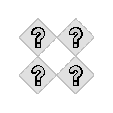
\includegraphics[scale=1]{0e0p/0e0p_double_transition_1.pdf}} \vcenteredhbox{\color{black}{$\xrightarrow[N]{\text{\clock{0}{1} 1}}$}} \vcenteredhbox{\patternimg{0.35}{0e0p_double_transition_2}}
		\caption{In the emulating CA, each $3 \times 3$ grid evolves in the same way over the course of $2$ generations, by evolving $2 \times 2$ grids individually.}
		\label{fig:0e0p_double_transition_em}
	\end{subfigure}
	\caption{The $8$-state CA that we construct will work by acting on $2 \times 2$ grids of cells in such a way that applying it twice results in the same evolution (at half speed) as applying the original $2$-state CA to $3 \times 3$ grids of cells.}\label{fig:0e0p_double_transition}
\end{figure}

While there are many ways that we could construct $N$, one reasonably simply approach is to ensure that if all four of its inputs comes from $\{0,7\}$ then its output is in $\{0,1,2,3,4,5,6\}$, and vice-versa. That is, we design the $8$-state CA so that patterns in even generations consist entirely of cells in the states $0$ and $7$, thus emulating the ``dead'' and ``live'' cells in a $2$-state CA, whereas in odd generations they consist entirely of cells in the states $0$ through $6$, which are just used as helper states for reconstructing the proper configuration in even generations.

We first specify how $N$ should act when all of the inputs that it receives are either $0$ or $7$. Since there are only $2^4 = 16$ possible combinations of inputs in this case, we can list how $N$ acts on them explicitly:
\begin{align}\label{eq:0e0p_N_from_even}
	\begin{aligned}
		N(0,0,0,0) & = 0, \\ N(0,0,7,0) & = 4, \\ N(0,0,0,7) & = 6, \\ N(0,0,7,7) & = 1,
	\end{aligned} && \begin{aligned}
		N(7,0,0,0) & = 1, \\ N(7,0,7,0) & = 5, \\ N(7,0,0,7) & = 4, \\ N(7,0,7,7) & = 6,
	\end{aligned} && \begin{aligned}
		N(0,7,0,0) & = 2, \\ N(0,7,7,0) & = 6, \\ N(0,7,0,7) & = 3, \\ N(0,7,7,7) & = 5,
	\end{aligned} && \begin{aligned}
		N(7,7,0,0) & = 3, \\ N(7,7,7,0) & = 4, \\ N(7,7,0,7) & = 0, \\ N(7,7,7,7) & = 2.
	\end{aligned}
\end{align}
These $16$ evolution rules are displayed in Figure~\ref{fig:0e0p_rule_em}, and they do not depend at all on the rule that we are trying to emulate (i.e., these input-output combinations of $N$ are the same no matter what $M$ is).

\begin{figure}[!htb]
	\centering
	\vcenteredhbox{\patternimg{0.35}{rule_em_0000_0}}\vcenteredhbox{\color{black}{$\xrightarrow{\text{\clock{0}{1}}}$}} \vcenteredhbox{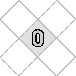
\includegraphics[scale=1]{0e0p/0e0p_rule_em_7077.pdf}} \hfill \vcenteredhbox{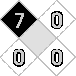
\includegraphics[scale=1]{0e0p/0e0p_rule_em_0007_0.pdf}}\vcenteredhbox{\color{black}{$\xrightarrow{\text{\clock{0}{1}}}$}} \vcenteredhbox{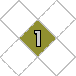
\includegraphics[scale=1]{0e0p/0e0p_rule_em_0007.pdf}} \hfill \vcenteredhbox{\patternimg{0.35}{rule_em_0070_0}}\vcenteredhbox{\color{black}{$\xrightarrow{\text{\clock{0}{1}}}$}} \vcenteredhbox{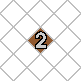
\includegraphics[scale=1]{0e0p/0e0p_rule_em_0070.pdf}} \hfill \vcenteredhbox{\patternimg{0.35}{rule_em_0077_0}}\vcenteredhbox{\color{black}{$\xrightarrow{\text{\clock{0}{1}}}$}} \vcenteredhbox{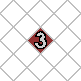
\includegraphics[scale=1]{0e0p/0e0p_rule_em_0077.pdf}} \\[1em]
	\vcenteredhbox{\patternimg{0.35}{rule_em_0700_0}}\vcenteredhbox{\color{black}{$\xrightarrow{\text{\clock{0}{1}}}$}} \vcenteredhbox{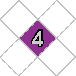
\includegraphics[scale=1]{0e0p/0e0p_rule_em_0700.pdf}} \hfill \vcenteredhbox{\patternimg{0.35}{rule_em_0707_0}}\vcenteredhbox{\color{black}{$\xrightarrow{\text{\clock{0}{1}}}$}} \vcenteredhbox{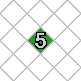
\includegraphics[scale=1]{0e0p/0e0p_rule_em_0707.pdf}} \hfill \vcenteredhbox{\patternimg{0.35}{rule_em_0770_0}}\vcenteredhbox{\color{black}{$\xrightarrow{\text{\clock{0}{1}}}$}} \vcenteredhbox{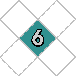
\includegraphics[scale=1]{0e0p/0e0p_rule_em_0770.pdf}} \hfill \vcenteredhbox{\patternimg{0.35}{rule_em_0777_0}}\vcenteredhbox{\color{black}{$\xrightarrow{\text{\clock{0}{1}}}$}} \vcenteredhbox{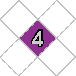
\includegraphics[scale=1]{0e0p/0e0p_rule_em_0700.pdf}} \\[1em]
	\vcenteredhbox{\patternimg{0.35}{rule_em_7000_0}}\vcenteredhbox{\color{black}{$\xrightarrow{\text{\clock{0}{1}}}$}} \vcenteredhbox{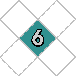
\includegraphics[scale=1]{0e0p/0e0p_rule_em_0770.pdf}} \hfill \vcenteredhbox{\patternimg{0.35}{rule_em_7007_0}}\vcenteredhbox{\color{black}{$\xrightarrow{\text{\clock{0}{1}}}$}} \vcenteredhbox{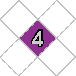
\includegraphics[scale=1]{0e0p/0e0p_rule_em_0700.pdf}} \hfill \vcenteredhbox{\patternimg{0.35}{rule_em_7070_0}}\vcenteredhbox{\color{black}{$\xrightarrow{\text{\clock{0}{1}}}$}} \vcenteredhbox{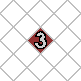
\includegraphics[scale=1]{0e0p/0e0p_rule_em_0077.pdf}} \hfill \vcenteredhbox{\patternimg{0.35}{rule_em_7077_0}}\vcenteredhbox{\color{black}{$\xrightarrow{\text{\clock{0}{1}}}$}} \vcenteredhbox{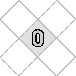
\includegraphics[scale=1]{0e0p/0e0p_rule_em_7077.pdf}} \\[1em]
	\vcenteredhbox{\patternimg{0.35}{rule_em_7700_0}}\vcenteredhbox{\color{black}{$\xrightarrow{\text{\clock{0}{1}}}$}} \vcenteredhbox{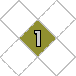
\includegraphics[scale=1]{0e0p/0e0p_rule_em_0007.pdf}} \hfill \vcenteredhbox{\patternimg{0.35}{rule_em_7707_0}}\vcenteredhbox{\color{black}{$\xrightarrow{\text{\clock{0}{1}}}$}} \vcenteredhbox{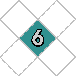
\includegraphics[scale=1]{0e0p/0e0p_rule_em_0770.pdf}} \hfill \vcenteredhbox{\patternimg{0.35}{rule_em_7770_0}}\vcenteredhbox{\color{black}{$\xrightarrow{\text{\clock{0}{1}}}$}} \vcenteredhbox{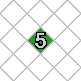
\includegraphics[scale=1]{0e0p/0e0p_rule_em_0707.pdf}} \hfill \vcenteredhbox{\patternimg{0.35}{rule_em_7777_0}}\vcenteredhbox{\color{black}{$\xrightarrow{\text{\clock{0}{1}}}$}} \vcenteredhbox{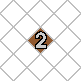
\includegraphics[scale=1]{0e0p/0e0p_rule_em_0070.pdf}}
	\caption{The rule for transitioning from even to odd generations in the $8$-state von-Neumann-neighborhood CA from Equation~\eqref{eq:0e0p_N_from_even}. The states $0$ and $7$ correspond to ``dead'' and ``alive'' in Life and are thus displayed in white and black, respectively. The states $1$, $2$, $3$, $4$, $5$, and $6$ are displayed in \bgbox{yellowback2}{yellow}, \bgbox{orangeback2}{orange}, \bgbox{redback}{red}, \bgbox{magentaback}{magenta}, \bgbox{greenpastel}{green}, and \bgbox{aquaback}{aqua}, respectively.}\label{fig:0e0p_rule_em}
\end{figure}

The reason for choosing these seemingly-random transition rules is that they lead to the function
\[
	\begin{pmatrix}
		a_{1,1} & a_{1,2} & a_{1,3} \\
		a_{2,1} & a_{2,2} & a_{2,3} \\
		a_{3,1} & a_{3,2} & a_{3,3}
	\end{pmatrix} \mapsto \begin{pmatrix}
		N\begin{pmatrix}
		a_{1,1} & a_{1,2} \\
		a_{2,1} & a_{2,2}
		\end{pmatrix} & N\begin{pmatrix}
		a_{1,2} & a_{1,3} \\
		a_{2,2} & a_{2,3}
		\end{pmatrix} \\
		N\begin{pmatrix}
		a_{2,1} & a_{2,2} \\
		a_{3,1} & a_{3,2}
		\end{pmatrix} & N\begin{pmatrix}
		a_{2,2} & a_{2,3} \\
		a_{3,2} & a_{3,3}
		\end{pmatrix}
	\end{pmatrix}
\]
from $\{0,7\}^9$ to $\{0,1,2,3,4,5,6\}^4$ being injective (i.e., each output of the function corresponds to a \emph{unique} input).\footnote{However, the choices we made in Equation~\eqref{eq:0e0p_N_from_even} (or equivalently, Figure~\ref{fig:0e0p_rule_em}) are not the only ones that lead to this function being injective. This collection of outputs, and many others, can be found by computer search---see Exercise~??.} That is, given any $2 \times 2$ arrangement of states $0$, $1$, $\ldots$, $6$, we can figure out which $3 \times 3$ arrangement of $0$ and $7$ states (if any) gave rise to it. We can thus define $N$ on inputs from $\{0,1,2,3,4,5,6\}^4$ so that Equation~\eqref{eq:0e0p_N_from_M} holds (i.e., the cellular automaton defined by $N$ emulates the cellular automaton defined by $M$ at half speed).

The resulting function $N$ is typically quite messy to write out in full detail (as it would just be an explicit list of how the $2^9 = 512$ possible arrangements of $2 \times 2$ grids of states $0$, $1$, $\ldots$, $6$ should evolve), even if the rule $M$ describes a relatively simple cellular automaton like Life. However, it can be constructed straightforwardly by a computer script,\footnote{One such script is available at \httpsurl{conwaylife.com/forums/viewtopic.php?p=38032}.} and the emulation of a glider in this way is illustrated in Figure~\ref{fig:0e0p_rule_em_glider}.

\begin{figure}[!htb]
	\centering
	\embedlink{0e0p_rule_em_glider}{\vcenteredhbox{\hphantom{${}\, \cdots$ \genarrow{1}}}\vcenteredhbox{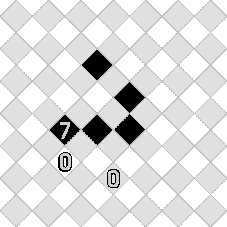
\includegraphics[scale=1]{0e0p/0e0p_glider_states0.pdf}} \vcenteredhbox{\genarrow{1}} \vcenteredhbox{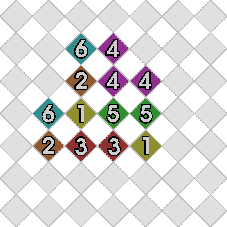
\includegraphics[scale=1]{0e0p/0e0p_glider_states.pdf}} \vcenteredhbox{\genarrow{1}} \vcenteredhbox{\patternimg{0.3}{0e0p_rule_em_glider_2}} \\[0.7em]
	\vcenteredhbox{$\cdots$ \genarrow{1}} \vcenteredhbox{\patternimg{0.3}{0e0p_rule_em_glider_3}} \vcenteredhbox{\genarrow{1}} \vcenteredhbox{\patternimg{0.3}{0e0p_rule_em_glider_4}} \vcenteredhbox{\genarrow{1}} \vcenteredhbox{\patternimg{0.3}{0e0p_rule_em_glider_5}} \\[0.7em] \vcenteredhbox{$\cdots$ \genarrow{1}} \vcenteredhbox{\patternimg{0.3}{0e0p_rule_em_glider_6}} \vcenteredhbox{\genarrow{1}} \vcenteredhbox{\patternimg{0.3}{0e0p_rule_em_glider_7}} \vcenteredhbox{\genarrow{1}} \vcenteredhbox{\patternimg{0.3}{0e0p_rule_em_glider_8}}}
	\caption{A glider from Life being emulated at half speed via an $8$-state cellular automaton using the von Neumann neighborhood (rotated by 45 degrees). Uses the same state coloring as in Figure~\ref{fig:0e0p_rule_em}, which describes the transitions from even to odd generations. The transitions from odd to even generations are encoded as an explicit list of which $2 \times 2$ arrangements of states $0$, $1$, $\ldots$, $6$ should lead to their central cell being born.}\label{fig:0e0p_rule_em_glider}
\end{figure}

The 0E0P metacell can be programmed to emulate any of the $8^{8^4-1}$ possible zero-preserving 8-state von-Neumann-neighborhood cellular automata in which every cell dies every generation (not just the ones that emulate one of the $2^{2^9-1}$ zero-preserving 2-state Moore-neighborhood CAs that we are actually interested in). It takes $2^{35}$ generations for the 0E0P metacell to run one generation of the 8-state rule (emulated at a 45-degree angle, as in the figures of this section), and therefore $2^{36}$ generations to emulate one generation of the corresponding 2-state Moore-neighborhood rule (in the usual orientation).


%%%%%%%%%%%%%%%%%%%%%%%%%%%%%%%%%%%
\section{Overview of the Metacell}\label{sec:0e0p_structure}
%%%%%%%%%%%%%%%%%%%%%%%%%%%%%%%%%%%

The 0E0P metacell works by using the single-channel glider synthesis techniques of Chapter~\ref{chp:universal_construction} to construct copies of itself in neighboring locations. It starts by constructing a copy to the southeast, northeast, northwest, and southwest (in that order, and only if no metacells are already present in those locations), and then it sends information about its current state to those neighboring metacells so that the proper rule is emulated.\index{single-channel synthesis}

In order to implement this behavior, the 0E0P metacell is made up of three components (see Figures~\ref{fig:0e0p_schematic} and~\ref{fig:0e0p_itself}), which are constructed by parent metacells one at a time:\smallskip

\begin{figure}[!htb]
	\centering
	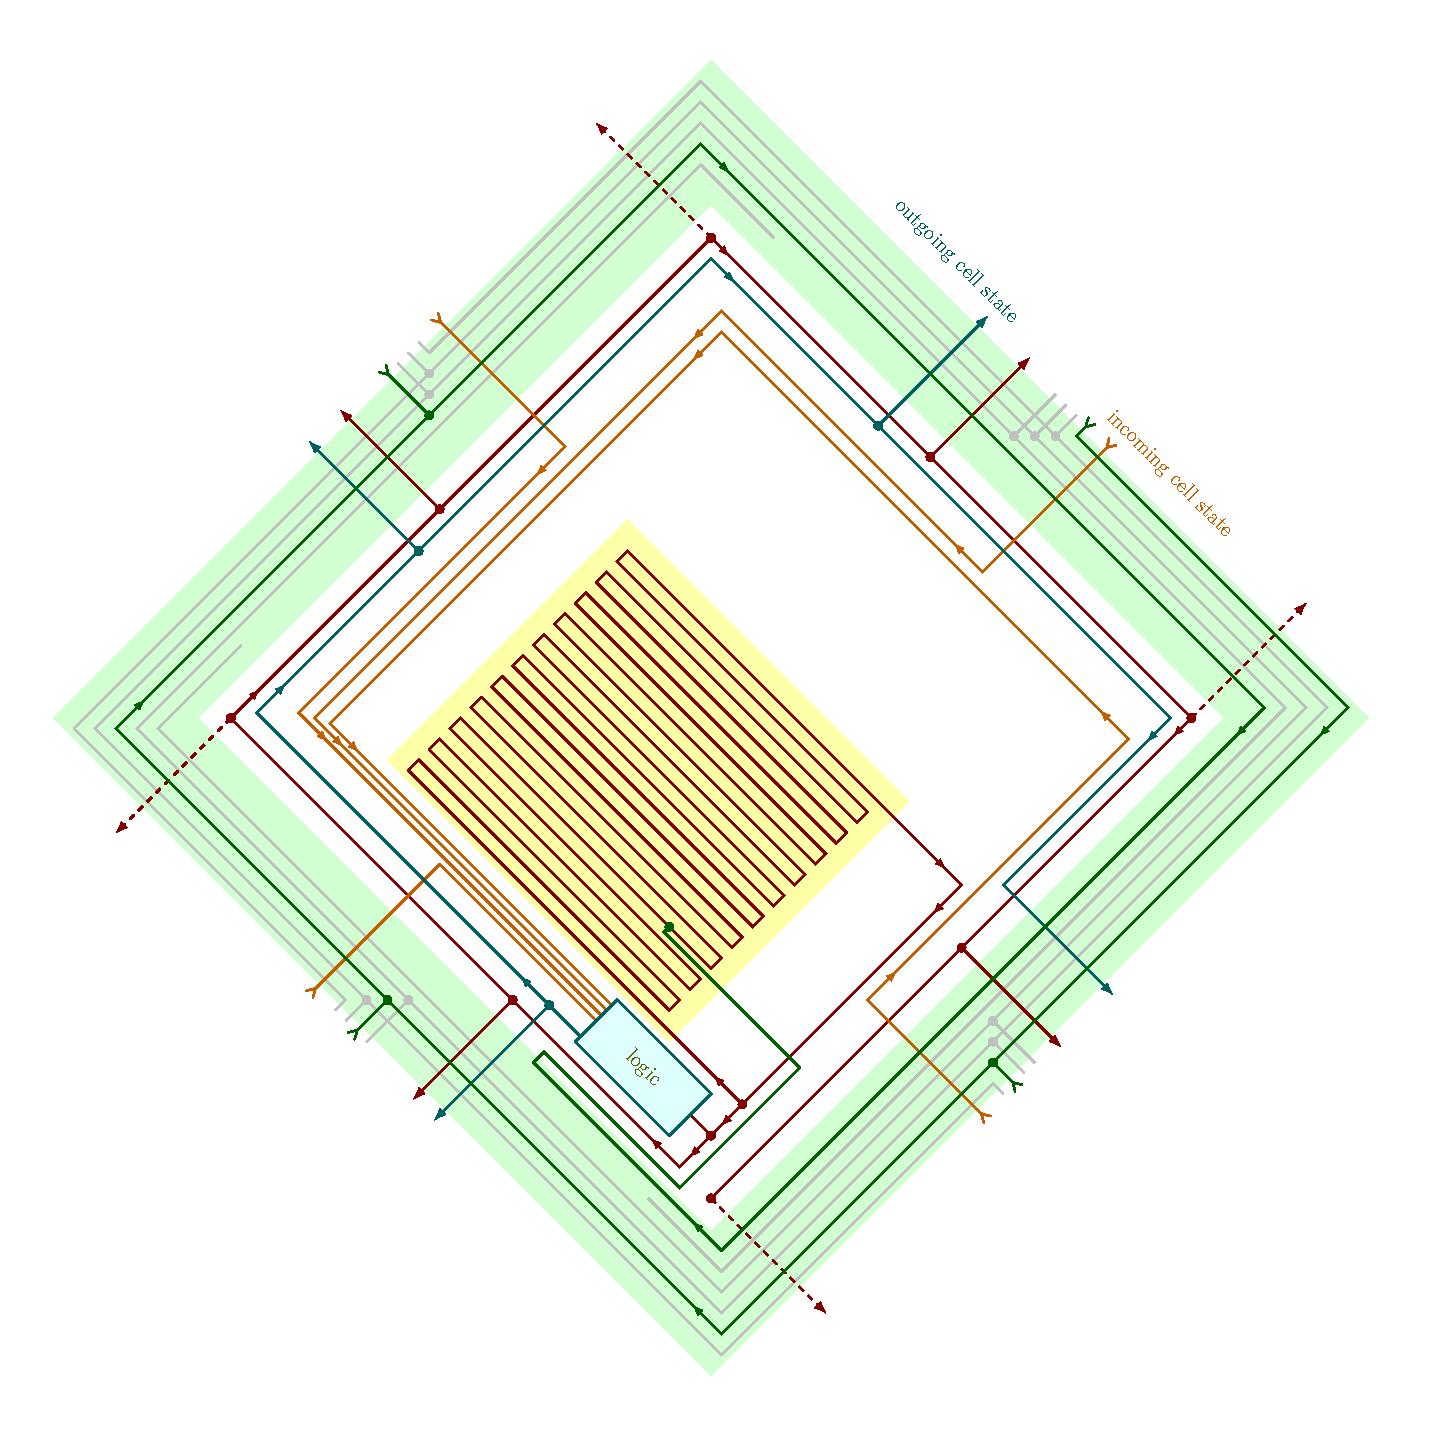
\includegraphics[width=\textwidth]{0e0p/0e0p_schematic.pdf}
	\caption{A schematic of the 0E0P metacell. The \textbf{nucleus}, highlighted in \bgbox{yellowback2}{yellow}, houses a single-channel glider sequence containing over 3~million gliders, which encode the rule being emulated as well as the construction of the 0E0P metacell itself. When the 0E0P is being constructed, its symmetrical outer \textbf{shell} (highlighted in \bgbox{greenpastel}{light green}) takes in the single-channel glider sequence from any of its neighboring parents (along the path displayed in \bgbox{greenback}{dark green}) and injects it into the nucleus. The unhighlighted region in the middle is the \textbf{kernel}, which contains an output path for a copy of the single-channel glider sequence (displayed in \bgbox{magentaback}{magenta}), as well as input and output paths along which parent metacells can tell child metacells what state they are in (displayed in \bgbox{orangeback2}{orange} and \bgbox{aquaback}{aqua}, respectively).}\label{fig:0e0p_schematic}
\end{figure}

\begin{figure}[!phtb]
	\centering
	\embedlink{0e0p}{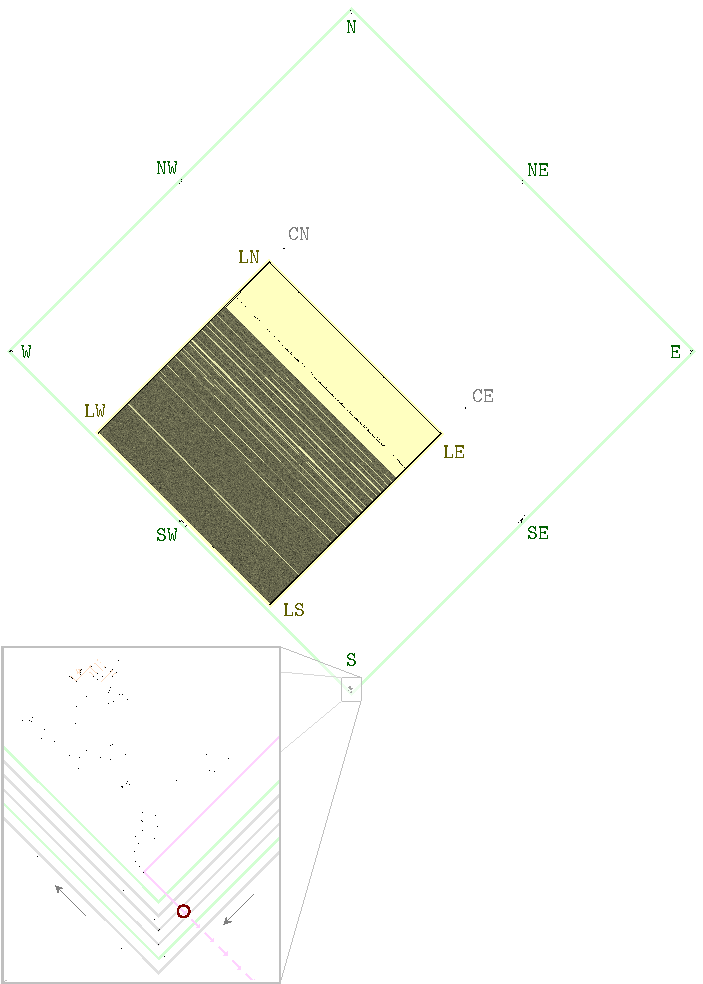
\includegraphics[width=\textwidth]{0e0p/0e0p.pdf}}	\caption{The 0E0P metacell itself, which implements the schematic of Figure~\ref{fig:0e0p_schematic}. It contains a significant amount of empty space between 14 points of interest. The shell (highlighted in \bgbox{greenpastel}{green}) goes through points \texttt{SW}, \texttt{W}, \texttt{NW}, \texttt{N}, \texttt{NE}, \texttt{E}, \texttt{SE}, and \texttt{S}, as do the points where the glider paths are reflected in the kernel. The logic circuitry is also located at point \texttt{S}, and an elbow block that is used to construct a new metacell to the southeast is circled in \bgbox{redback}{red}. The nucleus (highlighted in \bgbox{yellowback2}{yellow}) has corners at points \texttt{LW}, \texttt{LN}, \texttt{LE}, and \texttt{LS}. The sides between \texttt{LW} and \texttt{LN}, and between \texttt{LE} and \texttt{LS}, are each made up of $1{\thousep}024$ two-Snark (i.e., $180$-degree) reflectors that create a path long enough to house the nucleus's 3.6 million gliders. The points \texttt{CN} and \texttt{CE} are not displayed in the schematic of Figure~\ref{fig:0e0p_schematic}---they contain temporary circuitry that is used to construct the sides of the nucleus.}\label{fig:0e0p_itself}
\end{figure}
% TODO: Add more wires in the 2nd figure on 0E0P itself (i.e., not in the zoom box)?
% TODO: Show input and output orange/aqua wires to the logic component
% TODO: double-check S corner zoom box. At magenta corner on east side of logic component, gliders eventually pass through to the southwest, right? Seems to go to a slightly lower section of the SW component.

\begin{itemize}
	\item The outermost part is the \textbf{shell},\index{shell} which directs information about the states of neighboring metacells. It has exact 90-degree rotational symmetry, consisting of four spiral arms which propagate gliders inwards. Only one of these arms is actually used; the other four exist only to enforce the rotational symmetry.\smallskip
	
	\item Inside the shell is the \textbf{kernel},\index{kernel} which does not have any symmetry constraints. The south corner of the kernel contains a clock gun for regulating the metacell's lifecycle and logic circuitry for computing the state of the metacell based on the states of its four neighboring cells. The kernel also contains an output path, shown in magenta in Figure~\ref{fig:0e0p_schematic}, which can connect to one of the four construction arms (dashed) or to the input shell of one of the four neighbours.\smallskip
	
	\item At its center is the largest region of the metacell: its \textbf{nucleus},\index{nucleus} which is a huge boustrophedonic glider loop\footnote{That is, a glider loop in which the gliders travel back and forth along antiparallel lanes.} with a period of exactly $2^{29}$. It is populated by over three million gliders, which together encode a complete single-channel glider synthesis of the 0E0P metacell, along with a lookup table for the rule that the metacell is emulating.\smallskip
\end{itemize}

We describe how these three components of the metacell function throughout its lifecycle in more detail in the next three sections. We then talk about how they are constructed by parent metacells in Section~\ref{sec:0e0p_construction}.


%%%%%%%%%%%%%%%%%%%%%%%%%%%%%%%%%%%
\section{The Shell and Lane-Switching Circuitry}\label{sec:0e0p_structure_shell}\index{shell}
%%%%%%%%%%%%%%%%%%%%%%%%%%%%%%%%%%%

The rotationally symmetric shell that makes up the outermost edges of the 0E0P metacell is the simplest of its three components. Each of its four sides has four input lanes (in green and grey in Figure~\ref{fig:0e0p_schematic}). However, only one of these four input lanes is ever actually used (in green)---the one that connects to the output lane coming in from the kernel of the neighboring metacell (in solid magenta), if it exists.\footnote{This design is similar to that of a circuit on a motherboard---you can think of each side of the 0E0P metacell as having 8 ``pins'' (4 inputs pins and 4 output pins) that connect to the 8 pins of neighboring metacells.} The remaining input lanes (in grey) are unused, and only exist to enforce the shell's fourfold rotational symmetry.

After the metacell has been constructed, these input lanes read in a copy of the 0E0P's single-channel construction recipe and rule lookup table from its neighbors. That (extremely long) sequence of gliders revolves clockwise all the way around the spiral arm of the shell, until it is finally injected into the nucleus at the 0E0P's center.

To make sure that just one copy of the single-channel glider sequence is allowed to enter the shell, regardless of how many neighbors try to send in that glider sequence, the 0E0P strategically deletes part of its own circuitry after the nucleus is populated. By using a stray glider to delete a single block from a syringe, as demonstrated in Figure~\ref{fig:syringe_delete_block}, the 0E0P can change a syringe-based-reflector into a device that simply eats a glider stream. Another stray glider could also be used to destroy the syringe's eater~2, thus unblocking the stream as demonstrated in Figure~\ref{fig:syringe_delete_eater}, if desired.\footnote{This is not desired here, but we will see shortly that it is desired at another location in the 0E0P's circuitry.} These extra stray gliders are provided by its clock gun, which we discuss in the upcoming Section~\ref{sec:0e0p_structure_clock}.

% TODO: Be more specific about "shortly" in the above footnote. Reference a figure or section or something.

\begin{figure}[!htb]
	\centering
	\begin{subfigure}{.535\textwidth}
		\centering
		\embedlink{syringe_path_changer}{\vcenteredhbox{\patternimg{0.12}{syringe_delete_block}} \vcenteredhbox{\genarrow{120}} \vcenteredhbox{\patternimg{0.12}{syringe_delete_block_1}}}
		\caption{A single glider coming in from the southwest destroys a block, thus ``shutting off'' the syringe-based reflector.}
		\label{fig:syringe_delete_block}
	\end{subfigure} \hfill \begin{subfigure}{.435\textwidth}
		\centering
		\patternlink{syringe_path_changer}{\vcenteredhbox{\patternimg{0.12}{syringe_delete_eater}} \vcenteredhbox{\genarrow{120}} \vcenteredhbox{\patternimg{0.12}{syringe_delete_eater_1}}}
		\caption{A glider coming in from the northeast destroys the eater~2, thus unblocking the glider stream.}
		\label{fig:syringe_delete_eater}
	\end{subfigure}
	\caption{Some ways of deleting pieces of a syringe (displayed in \bgbox{redback}{red}) so as to change the path of a glider stream.}\label{fig:syringe_path_changer}
\end{figure}


%%%%%%%%%%%%%%%%%%%%%%%%%%%%%%%%%%%
\section{The Kernel}\label{sec:0e0p_structure_kernel}\index{kernel}
%%%%%%%%%%%%%%%%%%%%%%%%%%%%%%%%%%%

The asymmetric kernel contains the paths that are used to feed the 0E0P's single-channel recipe into its neighbors (in magenta in Figure~\ref{fig:0e0p_schematic}). Along these paths, gliders spiral clockwise-and-outwards, and then bypass the shell and do one of two things: go into a construction lane (in dashed magenta) to construct a neighboring metacell, or go into an output lane (in solid magenta) that connects to an input lane of an already-constructed neighboring metacell.

One important aspect of how the output and input lanes (not the construction lanes) of neighboring metacells connect to each other is that, irrespective of the orientation of the neighbors that are communicating, the single-channel glider sequence performs exactly 6 spiral quarter-turns to get from the south corner of the parent metacell to the south corner of the child metacell. This is how child metacells always end up in the correct phase and orientation after they are constructed.

In order to control which lane the single-channel glider sequence enters, the 0E0P periodically destroys some of the kernel's Snarks. We saw one method of doing this back in Figure~\ref{fig:snark_seeded_destroy}---a single glider can be used to destroy a Snark (with the help of 3 extra pre-placed still lifes). The 0E0P metacell makes use of Snark-destroying reactions like this one\footnote{But not \emph{exactly} this one---see Exercise~\ref{exer:0e0p_snark_destroyer}.} so as to redirect copies of its single-channel glider sequence to eight different locations over the course of its lifespan. In order,\footnote{The single-channel glider sequence really does have to be sent along these $8$ paths one after another. If we just used glider duplicators to send it along all $8$ paths at the same time, there could be unwanted collisions when constructing child metacells (e.g., if two parent metacells tried to create a child in the same location at the same time).} they are:\smallskip

\begin{itemize}
	\item[1)] Along the southeast construction lane (in dashed magenta in Figure~\ref{fig:0e0p_schematic}), to construct the child metacell to the southeast.\smallskip
	
	\item[2)] Along the southeast output lane (in solid magenta), to copy the glider sequence into the (now constructed) southeast child's nucleus.\smallskip
	
	\item[3)] Along the northeast construction lane (in dashed magenta), to construct the child metacell to the northeast.\smallskip
	
	\item[4) -- 8)] Along the northeast output lane, then the northwest construction lane, and so on counterclockwise.
\end{itemize}


%%%%%%%%%%%%%%%%%%%%%%%%%%%%%%%%%%%
\subsection{The Clock Gun}\label{sec:0e0p_structure_clock}\index{clock!gun}
%%%%%%%%%%%%%%%%%%%%%%%%%%%%%%%%%%%

The lane-switching mechanisms described earlier are implemented by a \textbf{clock gun} that is located at the top-left corner of the ``\texttt{logic}'' component in Figures~\ref{fig:0e0p_schematic} and~\ref{fig:0e0p_itself}. This gun sends out a single glider every $2^{29}$ generations, thus matching exactly the period of the glider loop contained in the nucleus. It is made up of a p256 gun attached to a sequence of $21$ semi-Snarks, much like the clock gun of Figure~\ref{fig:p2to_the_20_gun} that was used by Chapter~\ref{chp:universal_computation}'s universal computer (though that gun used quadri-Snarks instead).\footnote{The 0E0P's clock gun uses the color-changing semi-Snark of Figure~\ref{fig:cc_semi_snark}, since it is Spartan and is thus easier to construct via a single-channel glider recipe than quadri-Snarks.}\index{semi-Snark}\index{Spartan}

The gliders that are released by the clock gun travel through sequences of one-time turners and splitters that are interspersed throughout the rest of the 0E0P's circuitry, so as to the trigger the appropriate lane-switching mechanisms at each step of its lifecycle. This method is illustrated at a much smaller scale in Figure~\ref{fig:clock_path_switcher}, where a clock gun is used to change what happens to the path of a single-channel glider sequence three times.

\begin{figure}[!htb]
	\centering
	\embedlink{clock_path_switcher}{\vcenteredhbox{\hphantom{${}\ {}$ \genarrow{20}}}\vcenteredhbox{\patternimg{0.105}{clock_path_switcher_0}} \vcenteredhbox{\color{black}{$\xrightarrow{\text{\clock{4}{45} $2^{12}$}}$}} \vcenteredhbox{\patternimg{0.105}{clock_path_switcher_1}} \\[0.7em]
	\vcenteredhbox{\color{black}{$\xrightarrow{\text{\clock{4}{45} $2^{12}$}}$}} \vcenteredhbox{\patternimg{0.105}{clock_path_switcher_2}} \vcenteredhbox{\color{black}{$\xrightarrow{\text{\clock{4}{45} $2^{12}$}}$}} \vcenteredhbox{\patternimg{0.105}{clock_path_switcher_3}}}
	\caption{A period~$2^{12} = 4{\thousep}096$ clock gun (highlighted in \bgbox{aquaback}{aqua}) using one-time turners and the reactions from Figures~\ref{fig:snark_seeded_destroy} and~\ref{fig:syringe_path_changer} to change the path of the single-channel glider stream coming from the northwest. Initially, that stream is reflected to the northeast, but the first glider from the clock gun blocks the reflector. Its second glider unblocks it and redirects the stream to the southwest via a Snark. Its third glider destroys the Snark, so the stream passes straight through to the southeast.}\label{fig:clock_path_switcher}
\end{figure}

% EVERYTHING AFTER THIS POINT IS PLACEHOLDER and/or copied from forums and/or gibberish that will be changed

% Probably move all of the next few paragraphs earlier

There are some trombone slides of different lengths on different edges of the kernel, designed to compensate for the 'Olympic running track' effect where outer lanes of the spiral are disadvantaged vis-a-vis inner lanes. This ensures that the communication time from the parent to each of the four children is exactly the same.

Incoming gliders entering the child metacell get a 'head start', being injected several rows beyond the start of the tape. This 'head start' exactly compensates for the delay incurred by the gliders spiralling through the circuitry to pass from the parent metacell to the child, so the tapes of the parent and child metacell end up in exactly the same phase. This injection point is what you called 'Area 51' on Ch91's thread:

% Talk about the clock and show example figure of it implementing the single-channel-switching stuff from earlier

% Note to self: big gap in nucleus corresponds to when child metacell is repeatedly creating its nucleus's Snark loops. (i.e., when the child C1 and C2 are in use)
% Timeline file goes through 1.5*2^29 generations (i.e., 1.5 cycles of nucleus loop). 3072 snapshots at a spacing of 2^11 generations
% What happens during the 64 iterations of the glider loop during the 0E0P's life cycle? 1: construct SE, 2: copy into SE, 3: ?

% TODO: At start of "Overview of Metacell" section, give a warning that reader REALLY needs to try actually viewing 0E0P to get anything out of this. Mention its size, warn again that it is too slow to actually run, and give link to timeline files.


%%%%%%%%%%%%%%%%%%%%%%%%%%%%%%%%%%%
\subsection{Logic Circuitry}\label{sec:0e0p_structure_logic}
%%%%%%%%%%%%%%%%%%%%%%%%%%%%%%%%%%%

The kernel also contains, at its southern corner, the logic circuitry that is used to compute the metacell's state from the states of its four neighboring parents.

% Discuss the logic circuitry.
% We should have a big zoomed-in figure of the "logic" component.


%%%%%%%%%%%%%%%%%%%%%%%%%%%%%%%%%%%
\section{The Nucleus and Memory Tape}\label{sec:0e0p_structure_nucleus}\index{nucleus}
%%%%%%%%%%%%%%%%%%%%%%%%%%%%%%%%%%%

% In memory tape: roughly 3.5 million gliders in 3 groups
% 2465 doing rule table, but that amount varies depending on the rule.
% The other 15k or so at the very front encode the construction of 2 Snarks and some one-time stuff. Not sure why it's separated off on its own yet.

This is one of the few optimisations I deemed necessary. (Without this idea of subroutines and parallel construction, the metacell's side-length would need to be increased by a factor of 8.)

The 0E0P memory unit is a boustrophedonic tape loop composed of 180-degree reflectors (each of which is a pair of Snarks together with some nearby seeds of destruction). Each of those 180-degree reflectors is quite expensive; the single-channel recipe is somewhere between 1 and 2 million ticks. If the recipes for these reflectors were all individually stored in the memory unit, there would be a significant problem: adding more rows to the memory unit would linearly increase the total length of the recipe that needs to be stored in the memory unit. To break even, it would be necessary to increase the width of each row of the memory unit so that it takes 2 million ticks for gliders to travel from one 180-degree reflector to the next, making the memory unit 524288fd wide!

A solution is to only store the recipe for a single 180-degree reflector in the tape, and to repeatedly invoke this 'subroutine' in a loop. Due to parity constraints, the north-west and south-east 180-degree reflectors have a different shape, so it is necessary to have two 2-million-tick subroutines: one for the north-west reflectors, and one for the south-east reflectors. In the last phase of constructing the daughter metacell, these subroutines are injected into two small temporary memory loops. The two subroutines run in parallel (giving a 2x speedup compared with constructing the reflectors sequentially), and each loop has a fourfold fanout to construct four copies of the same reflector simultaneously. The effect is that the memory loop is constructed in one-eighth of the time necessary for sequential synthesis, so the memory unit can be a mere 65536fd wide.

This reduces the problem of constructing an immense ($2^{29}$-tick) memory loop to the problem of constructing two smaller memory loops ($2^{21}$ ticks each) to handle the subroutines. These smaller memory loops are small enough that they can be built in a naive sequential manner along with the remainder of the kernel of the 0E0P metacell. The small memory loops are each equipped with a binary counter which halts the subroutine after it has run for exactly 256 iterations and built 1024 reflectors (i.e. 2048 Snarks).

These subroutine storage units are among the most complicated mechanisms in the 0E0P metacell. A lot of the rest of the 0E0P recipe is just simple single-channel recipes, building one thing after another after another. But for these two storage units it's necessary to extract two small pieces of the full recipe, and execute each one 512 times to build the Snark chains that make up the "nucleus". Adam mentioned that the 0E0P would have had to be a lot bigger if the recipes for all of those Snarks were included inline with no subroutines


%%%%%%%%%%%%%%%%%%%%%%
\section{Construction}\label{sec:0e0p_construction}
%%%%%%%%%%%%%%%%%%%%%%

Ensuring all four metacells are built in the same orientation is by building the outer shell first (which is impossible to get wrong, because it's rotationally symmetric!) and then sending the remainder of the recipe through the correct pin to build the kernel in the correct orientation. If we'd counterfactually sent gliders down one of the other three pins, they'd end up in a different one of the four spiral arms and the resulting metacell would be in the wrong orientation.

% nucleus period 2^29, cycles 2^6 = 64 times to give full period of 2^35
% Mention cordership-push stuff here

% TODO: Have a figure like Stage 0 (yellow) showing the construction of a metacell up close in this section

% TODO: Followed by the 15-stage glider figure


%%%%%%%%%%%%%%%%%%%%%%
\section{A Complete Lifecycle}\label{sec:0e0p_timeline}
%%%%%%%%%%%%%%%%%%%%%%

So far, we have described how the 0E0P metacell works at a fairly high level: every $2^{29}$ generations, the clock gun fires a glider that potentially changes what happens throughout the metacell. Some of these gliders direct the single-channel glider sequence from the nucleus to start constructing a neighboring metacell, some of them redirect that glider sequence to be duplicated into a neighbor's nucleus, and some of them trigger the self-destruction of the entire metacell.

If we break the $2^{35}$-generation lifecycle of the metacell down into $2^6 = 64$ ``cycles'' of $2^{29}$ generations each, then they behave roughly as follows:\smallskip

\begin{itemize}
	\item Cycle 1: The metacell constructs its southeast neighbor.\smallskip
	
	\item Cycle 2: It duplicates the contents of its nucleus into that of the southeast neighbor.\smallskip
	
	\item Cycle 3: It constructs its northeast neighbor.\smallskip
	
	\item Cycle 4: It duplicates the contents of its nucleus into that of the northeast neighbor.\smallskip
	
	\item Cycles 5--8: Repeat cycles 1--4 for the northwest and then southwest neighbors.\smallskip
	
	\item Cycles 9--13: Do nothing (just spend some time ``looking like a cell'').\smallskip
	
	\item Cycle 14: The single-channel glider stream is emptied out of the metacell's nucleus. Simultaneously, information about the metacell's state is sent to all four of its neighbors.\smallskip
	
	\item Cycles 15--64: The parent metacell self-destructs and child metacells do nothing (they just spend some time ``looking like a cell'').\smallskip
\end{itemize}
% Can we be slightly more specific above? Does the self-destruction happen in cycle 15 exactly, for example?

% Timeline of important moments down here. Need to lead-in and reference these figures.

% To convert a timestamp from here to a timestamp from 0e0p_timeline.mc, add 138590856 = 33 * 2^22 + 178824


\clearpage

\newgeometry{top=28mm,left=28mm,bottom=0mm,right=28mm,headsep=10pt,a4paper}

\begin{figure}[!htb]
	\centering
	
	\embedlink{0e0p_timeline_0_small}{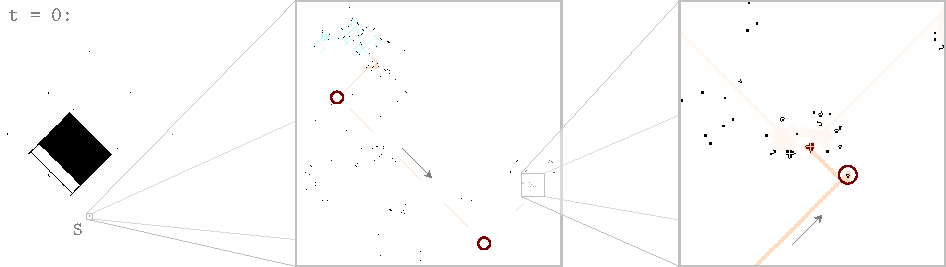
\includegraphics[width=1\textwidth]{0e0p/0e0p_timeline_0.pdf}}
	\caption{A Herschel in the parent metacell's clock gun (highlighted in \bgbox{aquaback}{aqua}) is about to create a glider that will make it all the way out of the clock. It will use some one-time turners (circled in \bgbox{redback}{red}) and then destroy an eater~2 from a syringe, which will allow a copy of the single-channel glider recipe to escape from the nucleus and start constructing the southeast child metacell, starting with its shell.}
	\label{fig:0e0p_timeline_0}
\end{figure}

\begin{figure}[!htb]
	\centering
	
	\vspace*{-0.3cm}
	
	\embedlink{0e0p_timeline_17367250_small}{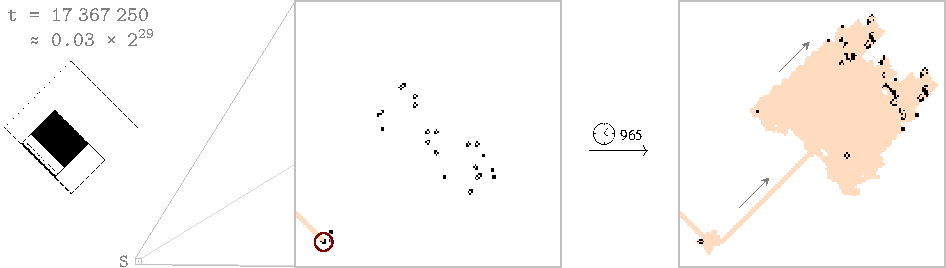
\includegraphics[width=1\textwidth]{0e0p/0e0p_timeline_17367250.pdf}}
	\caption{A glider (circled in \bgbox{redback}{red}) at the south corner of the child metacell's shell, about to synthesize a Cordership that does a long-distance elbow push to its east corner.}
	\label{fig:0e0p_timeline_17367250}
\end{figure}

\begin{figure}[!htb]
	\centering
	
	\vspace*{-0.3cm}
	
	\embedlink{0e0p_timeline_107585535_small}{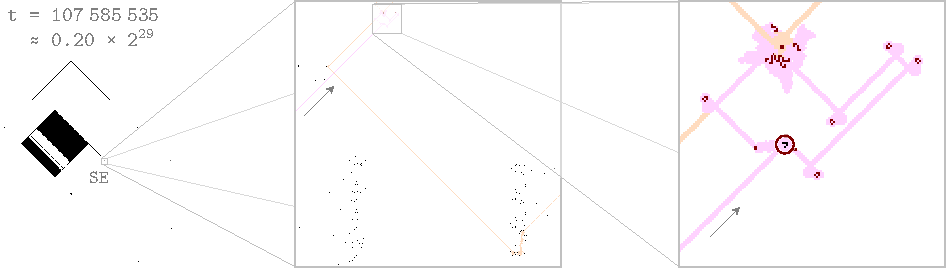
\includegraphics[width=1\textwidth]{0e0p/0e0p_timeline_107585535.pdf}}
	\caption{The southeast child's shell has been constructed. A single stray glider (circled in \bgbox{redback}{red}) is about to delete a Snark, allowing the rest of the construction recipe to enter the correct lane of the child's shell. This ensures that the rest of that child is constructed in the proper orientation.}
	\label{fig:0e0p_timeline_107585535}
\end{figure}

\begin{figure}[!htb]
	\centering
	
	\vspace*{-0.3cm}
	
	\embedlink{0e0p_timeline_334193646_small}{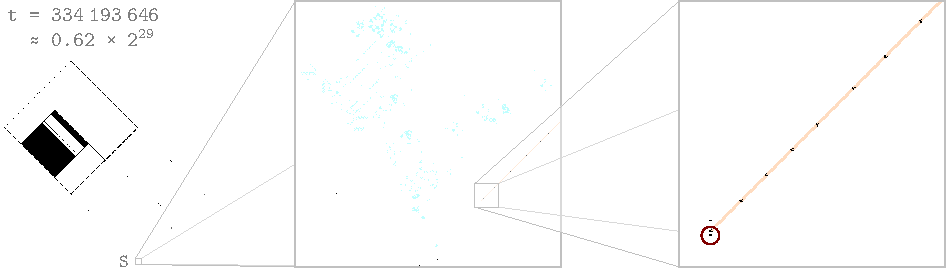
\includegraphics[width=1\textwidth]{0e0p/0e0p_timeline_334193646.pdf}}
	\caption{Construction of the child's south corner begins. The logic circuit (highlighted in \bgbox{aquaback}{aqua}, including the clock gun) will now be constructed by the elbow block circled in \bgbox{redback}{red}.}
	\label{fig:0e0p_timeline_334193646}
\end{figure}

\begin{figure}[!htb]
	\centering
	
	\embedlink{0e0p_timeline_397258593_small}{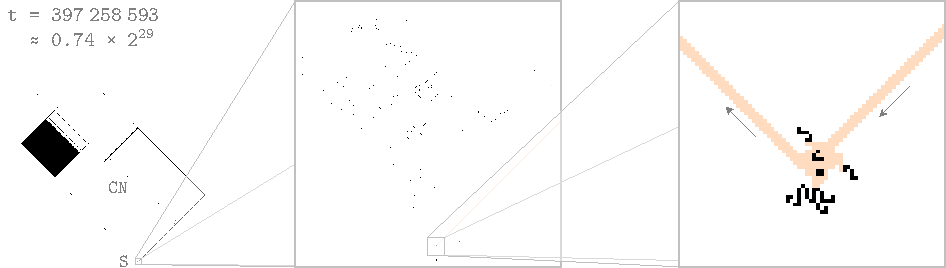
\includegraphics[width=1\textwidth]{0e0p/0e0p_timeline_397258593.pdf}}
	\caption{The child's kernel has been constructed. A glider goes through a brand new Snark at its south corner that leads it to \texttt{CN}, which will trigger construction of the nucleus walls.}
	\label{fig:0e0p_timeline_397258593}
\end{figure}

\begin{figure}[!htb]
	\centering
	
	\vspace*{-0.3cm}
	
	\embedlink{0e0p_timeline_398415184_small}{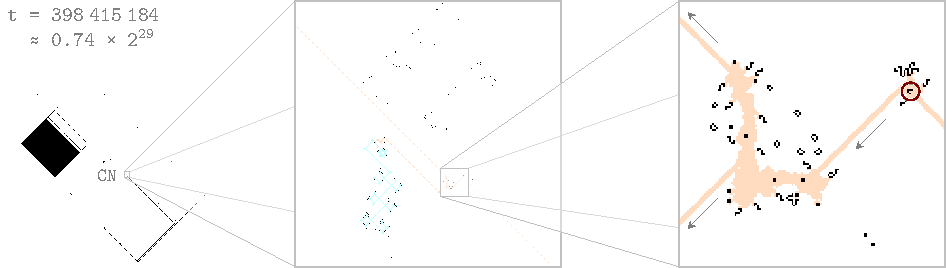
\includegraphics[width=1\textwidth]{0e0p/0e0p_timeline_398415184.pdf}}
	\caption{The glider from Figure~\ref{fig:0e0p_timeline_397258593} has reached \texttt{CN} and is about to start the clock there (highlighted in \bgbox{aquaback}{aqua}), which will trigger \texttt{CN}'s self-destruction $2^{29}$ generations later.}
	\label{fig:0e0p_timeline_398415184}
\end{figure}

\clearpage

\restoregeometry

% TODO: Check that the coordinates in the timestamp files themselves are correct (they were relative to linear_construct_canon.mc.gz, so they may have changed slightly)


%%%%%%%%%%%%%%%%%%%%%%%%%%%%%%%%
\section{Notes and Historical Remarks}\label{sec:0e0p_history}\index{metacell}
%%%%%%%%%%%%%%%%%%%%%%%%%%%%%%%%

Many metacells---patterns of size larger than $1 \times 1$ that emulate the behavior of a single cell---were constructed prior to 0E0P. The first one was the \textbf{p5760~metacell}, which was constructed by David Bell in January 1996. This metacell is much smaller and faster than 0E0P, with a period of just $5{\thousep}760$~generations and a bounding box size of just $500 \times 500$ (see Figure~\ref{fig:p5760_metacell}). However, there are numerous trade-offs that make this metacell less useful:\smallskip

\begin{figure}[!htb]
	\centering
	\begin{tikzpicture}
		\node[inner sep=0pt,anchor=south west] at (0,0) {\embedlink{p5760_metacell}{\patternimg{0.15}{p5760_metacell}}};
	
		\draw[white,line width=2.5pt,opacity=0.6](2.63,8.15) circle (0.2);
		\draw[redback2,line width=1pt](2.63,8.15) circle (0.2);
	\end{tikzpicture}
	\caption{The \emph{p$5760$~metacell}. Whether the cell is considered ``alive'' or ``dead'' is determined by the presence or absence of a glider at the location circled in \bgbox{redback}{red}. That glider, if present, is duplicated $8$ times and sent to its neighbors along the $8$ output paths highlighted in \bgbox{aquaback}{aqua}, signaling to them that it is alive. Similarly, neighboring alive cells send their signals to this one along the input paths highlighted in \bgbox{magentaback}{magenta}.}\label{fig:p5760_metacell}
\end{figure}

\begin{itemize}
	\item[1)] It is hard-wired to emulate Life, and cannot easily be modified to emulate most of the $2^{512}$ different non-isotropic Life-like cellular automata.\smallskip
	
	\item[2)] It is not easy to tell at a glance which ``cells'' are alive and which are dead---it is determined by the presence or absence of a single extra glider in the cell---and thus is not interesting to look at from a far-out zoom level.\smallskip
	
	\item[3)] ``Dead'' cells must be placed on the Life plane, which means that, for example, spaceships cannot be emulated by this metacell unless the pattern is infinitely large.\smallskip
\end{itemize}

The first two of these problems were solved by the \emph{OTCA metapixel},\index{OTCA metapixel} which was constructed by Brice Due from late 2005 to mid-2006. While this metacell is a bit larger and slower than the first metacell (it is $2048 \times 2048$ and has period $35{\thousep}328$), it can be used to emulate any of the $2^{18}$ different outer-totalistic Life-like cellular automata. Indeed, built into its circuitry is an easily-adjustable array of eaters that determine how many live neighboring OTCA metapixels should lead to the birth or survival of the current metapixel (see Figure~\ref{fig:otca_metapixel}). 
% Introduce Life-like CA, since no introduction earlier
% mention out of the blue/honey bit/demultiplexer?

% FIGURE HERE, SHOWING PIXEL AND RULE ENCODINGS

The OTCA metapixel also has the remarkable feature that its alive and dead states look, from a distance, like alive and dead cells. This feature is achieved by the ``alive'' version of the cell releasing $43$ pairs of perpendicular lightweight spaceship streams that mutually annihilate each other, thus partially filling in the otherwise empty center of the metacell. For example, arranging a $1 \times 3$ row of ``alive'' metapixels (and a suitably large ``dead'' array of metapixels around its edges) results in a pattern that looks and evolves like a blinker, but $2{\thousep}048$ times as long and wide and $35{\thousep}328$ times as slow (see Figure~\ref{fig:metablinker}).

\begin{figure}[!htb]
	\centering
	\embedlink{metablinker}{\vcenteredhbox{\patternimg{0.104}{metablinker_0}} \vcenteredhbox{\color{black}{$\xrightarrow{\text{\clock{5}{46} 35328}}$}} \vcenteredhbox{\patternimg{0.104}{metablinker_35328}}}
	\caption{A \emph{metablinker}: an arrangement of OTCA metapixels that emulates a blinker, but with period $2 \times 35{\thousep}328$.}\label{fig:metablinker}\index{metablinker}
\end{figure}

The next notable metacell to be constructed was the \emph{p1 megacell},\index{p1 megacell} by Adam P.~Goucher in 2008. This metacell was, again, larger and slower than the metacells that came before it, with a bounding box of $2^{15} \times 2^{15}$ and a period of $2^{24}$. The new features this time that warranted the extra size and delay were twofold:\smallskip

\begin{itemize}
	\item This metacell was built entirely out of stable (p$1$) components like Herschel tracks, with the exception of a single period~$2^{24}$ gun used to regulate its timing.\footnote{This gun could be swapped out for a gun of another period, but periods that are multiples of $2$ help the pattern run quicker under the HashLife algorithm in Life simulation software like Golly.}\index{HashLife}\smallskip
	
	\item All $2^{512}$ non-outer-totalistic Life-like cellular automata can be emulated by this metacell, versus the $2^{18}$ outer-totalistic Life-like cellular automata that can be emulated by the OTCA metapixel.\smallskip% Maybe not-necessarily-outer-totalistic, instead of non-outer-totalistic?
\end{itemize}

% Figure of p1 megacell? Have had a lot of big figures bunched up closely here, so maybe not.

Finally, Adam P.~Goucher spent 2014--2018 constructing the 0E0P metapixel, which solved problem~(3) described earlier---it does not require a background grid of ``dead'' cells to be placed on the Life plane.

%https://www.conwaylife.com/forums/viewtopic.php?f=15&t=4117#p82954
%https://cp4space.hatsya.com/2018/11/12/fully-self-directed-replication/
%https://www.conwaylife.com/forums/viewtopic.php?f=2&t=3835
%https://www.conwaylife.com/forums/viewtopic.php?t=3968
%https://www.conwaylife.com/forums/viewtopic.php?p=72241

% EXERCISE: Give reactions in HighLife-replicator-ship.rle from Golly and ask reader to make ship out of it
% EXERCISE: Logarithmic replicator from B36/S245, found by Mark Niemiec in July 1994. Do... something with it. Pop in generation 300*4^n - 127 is 64 for all n >= 0.

% EXERCISE: There is *almost* an RRO in a Life-like, but just give a footnote/exercise about it. Exercise could ask why it's not a true RRO.
% EXERCISE: Show how iso in Moore neighborhood can emulate outer totalistic in von Neumann neighborhood
% EXERCISE: Give iso rulestring for (some rule)
% EXERCISE: Create a non-iso rule in which a single cell acts as... (diagonal spaceship, what else?)
% Exercise about emulating an elementary cellular automaton

% EXERCISE(S) about transition rules for rule emulation: find another one. Also:
% the different cell states, there are 200 different such functions sending 0 to 0.
% With 8 states we have 7 colors. Doing this with 6 or fewer colours is absolutely impossible, and with 7 colours is difficult (there are only 200 distinct solutions, or 13 up to rotation/reflection).
% EXERCISE: Describe positions of replicators in HashLife replicator? Connect to Sierpinski triangle maybe (same pattern as n-th row of it)
% Maybe exercise about 89-rotational RRO (https://www.conwaylife.com/forums/viewtopic.php?f=15&t=4116&p=131063#p131063). Or a part (b) of the already-planned RRO exercise?


%%%%%%%%%%%%%%%%%%%%%%%%%%%%%%%%%
\section*{Exercises \hfill \normalfont\textsf{\small solutions to starred exercises on \hyperlink{solutions_0e0p}{page \pageref{solutions_0e0p}}}}
\label{sec:solutions_0e0p}
\addcontentsline{toc}{section}{Exercises}
\vspace*{-0.4cm}\hrulefill\vspace*{-0.3cm}\footnotesize\begin{multicols}{2}\vspace*{-0.4cm}\raggedcolumns\interlinepenalty=10000
	\setlength{\parskip}{0pt}
	%%%%%%%%%%%%%%%%%%%%%%%%%%%%%%%%%
	
	
	\begin{problem}\label{exer:replicator_rule_really_replicates}
		Recall the replicator rule \texttt{B1357/S1357} that was illustrated in Figure~\ref{fig:replicator_smile}.\smallskip
		
		\begin{enumerate}[label=\bf\color{ocre}(\alph*)]
			\item \probdiff{2} If the longest side of a pattern's bounding box is $n$ cells long, how many generations would it take to copy itself for the first time in this rule?
			% Solution: 2^(ceil(log_2(n))) generations
			
			\item \probdiff{5} Prove that every pattern in this rule really does replicate, as we claimed.
			
			\noindent [Hint: First, prove (via induction, perhaps) that a single cell replicates. Then show that evolving a multi-cell pattern in this rule is equivalent to evolving each cell individually and XOR-ing the results together.].
		\end{enumerate}
	\end{problem}


	\mfilbreak
	
	
	\begin{problem}\label{exer:0e0p_single_cell_spaceships}
		Modify the rule used in Figure~\ref{fig:single_cell_knightship} so as to construct a (non-isotropic) 2-state cellular automaton on a square grid in which a single cell is a spaceship with speed...\smallskip
		
		\begin{enumerate}[label=\bf\color{ocre}(\alph*)]
			\item \probdiff{2} $c/2$ orthogonal;
			
			\item \probdiff{2} $c$ diagonal;
			
			\item \probdiff{2} $c/2$ diagonal; and
			
			\item \probdiff{4} $(1,3)c/4$ or any other non-orthogonal, non-diagonal, and non-knightship slope.
			
			\noindent [Hint: Use two generations to transform the cell into a domino, and two more generations to transform it back into a single cell.]
		\end{enumerate}
	\end{problem}
% SOLUTIONS: https://www.conwaylife.com/forums/viewtopic.php?f=11&t=3089&p=95700&hilit=MAP#p96359
% MORE: https://www.conwaylife.com/forums/viewtopic.php?f=11&t=3089&hilit=MAP&start=50#p98128


	\mfilbreak
	
	
	\begin{problem}\label{exer:0e0p_rro_technicalities} \probdiff{3}
		Copies of the 0E0P metacell can be placed on the Life plane so as to evolve in the same way as the pattern from Figure~\ref{fig:reflectorless_rotating_oscillator1}.\smallskip
		
		\begin{enumerate}[label=\bf\color{ocre}(\alph*)]
			\item Explain why this pattern is \emph{not} a reflectorless rotating oscillator in Life, despite being a RRO in the rule that the 0E0P is emulating.
			% SOLUTION: metacell itself does not rotate
			
			\item Explain how you could use even more 0E0P metacells to emulate multiple copies of the pattern from Figure~\ref{fig:reflectorless_rotating_oscillator1} so as to create an actual RRO in Life.
			% Use four copies, rotated
		\end{enumerate}
	\end{problem}


	\mfilbreak


	\begin{problem}\label{exer:0e0p_one_cell_smos}\index{spaceship made of spaceships} \probdiff{3}
		Create a von-Neumann-neighbourhood cellular automaton on a 2D square grid with at most $8$ states, where every cell dies in every generation (so it is of the type described in Section~\ref{sec:0e0p_rule_emulation} that can be emulated by the 0E0P metacell), in which two single-cell spaceships can collide so as to create a $2$-cell SMOS.
		
		\noindent [Hint: Make a cell in one state move south, a cell in another state move east, and something else happen when they collide.]
	\end{problem}
	% SOLUTION: https://www.conwaylife.com/forums/viewtopic.php?p=72241#p72170


	\mfilbreak
	
	
	\begin{problem}\label{exer:non_isotropic_rulestring_life} \probdiff{3}
		What is the non-isotropic rulestring (in the sense of Appendix~\ref{sec:non_isotropic_rulestrings}) for Conway's Game of Life?
	\end{problem}
	% SOLUTION: MAPARYXfhZofugWaH7oaIDogBZofuhogOiAaIDogIAAgAAWaH7oaIDogGiA6ICAAIAAaIDogIAAgACAAIAAAAAAAA
	
	
	\mfilbreak
	
	
	\begin{problemstar}\label{exer:0e0p_snark_destroyer} \probdiff{2}
		Recall that a single glider can destroy a Snark, as long as we place some extra still lifes near it as in Figure~\ref{fig:snark_seeded_destroy}.\smallskip
		
		\begin{enumerate}[label=\bf\color{ocre}(\alph*)]
			\item Find a similar configuration of still lifes that is used in the 0E0P metacell so as to allow a single glider to destroy a Snark.
			
			\item Explain why the configuration of still lifes from part~(a) might be preferable to the one from Figure~\ref{fig:snark_seeded_destroy}, despite being larger.
		\end{enumerate}
	\end{problemstar}
	
	
	%% EXERCISE END COMMANDS
\end{multicols}
\normalsize\vspace*{0.01cm}
%% DONE EXERCISE END COMMANDS
